\documentclass{article}
\usepackage{tikz}
\usetikzlibrary{patterns,shadings}
\begin{document}
% 路径类型
% 1.描边线
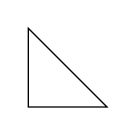
\begin{tikzpicture}
    %   \path[draw],可简写为\draw
    \path[draw] (0,0) -- (1,0) -- (0,1) -- cycle;
\end{tikzpicture}\vspace{1cm}


% 2.内容填充

\begin{tikzpicture}
    %   \path[fill],可简写为\fill
    %   可与draw参数一起使用,底层先fill,后draw
    %   必须为闭合线条
    \path[fill] (0,0) -- (1,0) -- (0,1) -- cycle;
\end{tikzpicture}\vspace{1cm}

% 同一命令,图形重叠部分的填充方式
% 1)nonzero rule
%   判断point是否在多层path内部,将point作为一个光源,并设置一个初始为0的数num
%   当发射的光碰到一层path时,如果路径方向(光的视角)为从左到右,则num加1;如果路径为从右到左,则num减1
%   在光到达path外部时,如果num不为0,则认为point在path内部(填充);为0,则在外部(不填充)
% 默认方式
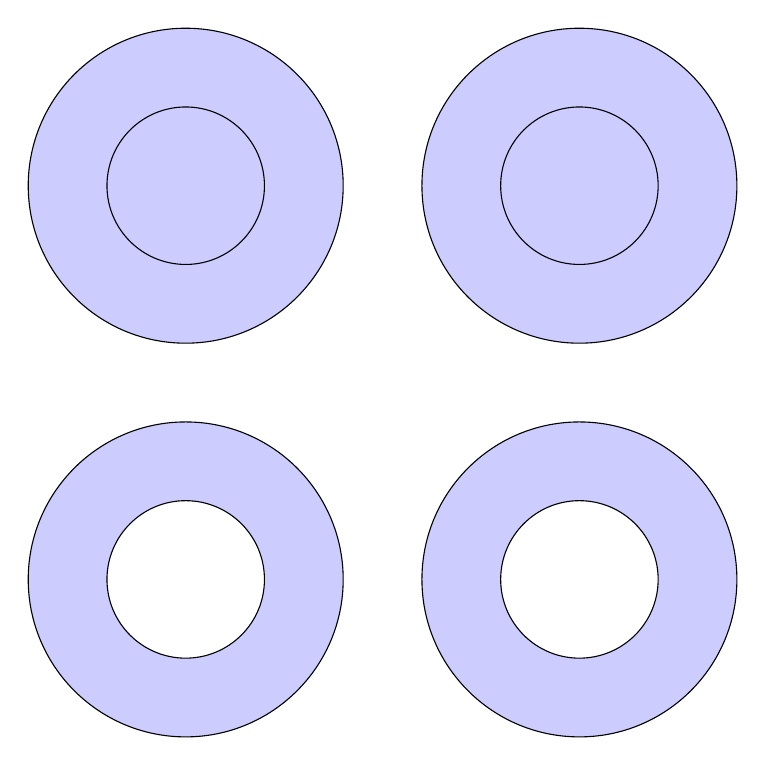
\begin{tikzpicture}
    \filldraw[fill=blue!20] (2,0) arc [start angle=0,end angle=360,radius=2] (1,0) arc [start angle=0,end angle=360,radius=1];
    \filldraw[fill=blue!20] (7,0) arc [start angle=360,end angle=0,radius=2] (6,0) arc [start angle=360,end angle=0,radius=1];
    \filldraw[fill=blue!20] (2,-5) arc [start angle=0,end angle=360,radius=2] (1,-5) arc [start angle=360,end angle=0,radius=1];
    \filldraw[fill=blue!20] (7,-5) arc [start angle=360,end angle=0,radius=2] (6,-5) arc [start angle=0,end angle=360,radius=1];
\end{tikzpicture}

% 2)even odd rule,图形相交部分直接留白
%   判断point是否在多层path内部,将point作为一个光源,并设置一个初始为0的数num
%   当发射的光碰到一层path时,如果路径方向(光的视角)为从左到右,则num加1;如果路径为从右到左,则num减1
%   在光到达path外部时,如果num为奇数,则认为point在path内部(填充);为偶数,则在外部(不填充)
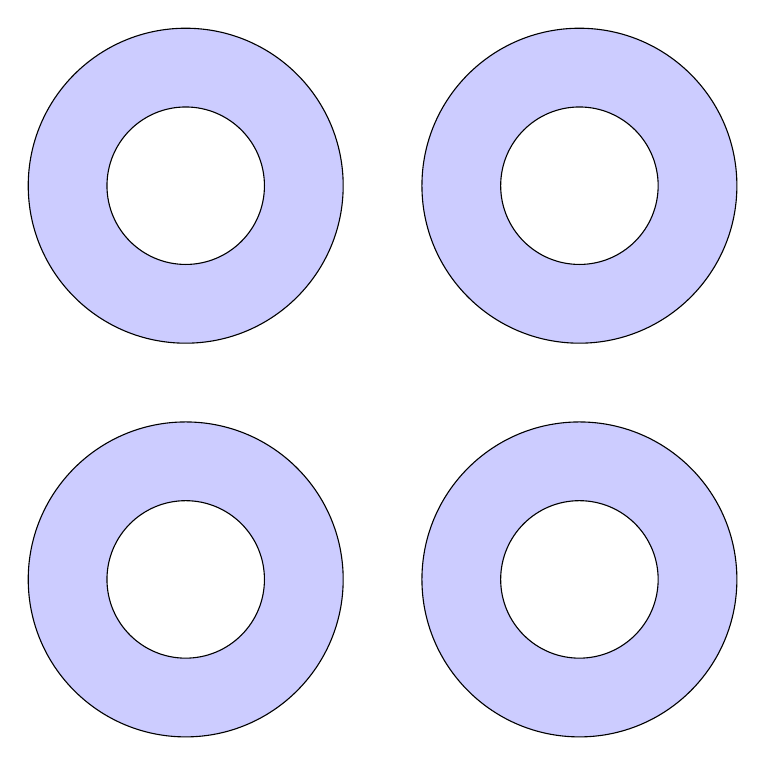
\begin{tikzpicture}
    \filldraw[fill=blue!20,even odd rule] (2,0) arc [start angle=0,end angle=360,radius=2] (1,0) arc [start angle=0,end angle=360,radius=1];
    \filldraw[fill=blue!20,even odd rule] (7,0) arc [start angle=360,end angle=0,radius=2] (6,0) arc [start angle=360,end angle=0,radius=1];
    \filldraw[fill=blue!20,even odd rule] (2,-5) arc [start angle=0,end angle=360,radius=2] (1,-5) arc [start angle=360,end angle=0,radius=1];
    \filldraw[fill=blue!20,even odd rule] (7,-5) arc [start angle=360,end angle=0,radius=2] (6,-5) arc [start angle=0,end angle=360,radius=1];
\end{tikzpicture}\newpage


% 3.填充内容从一个颜色平滑过渡到另一个颜色
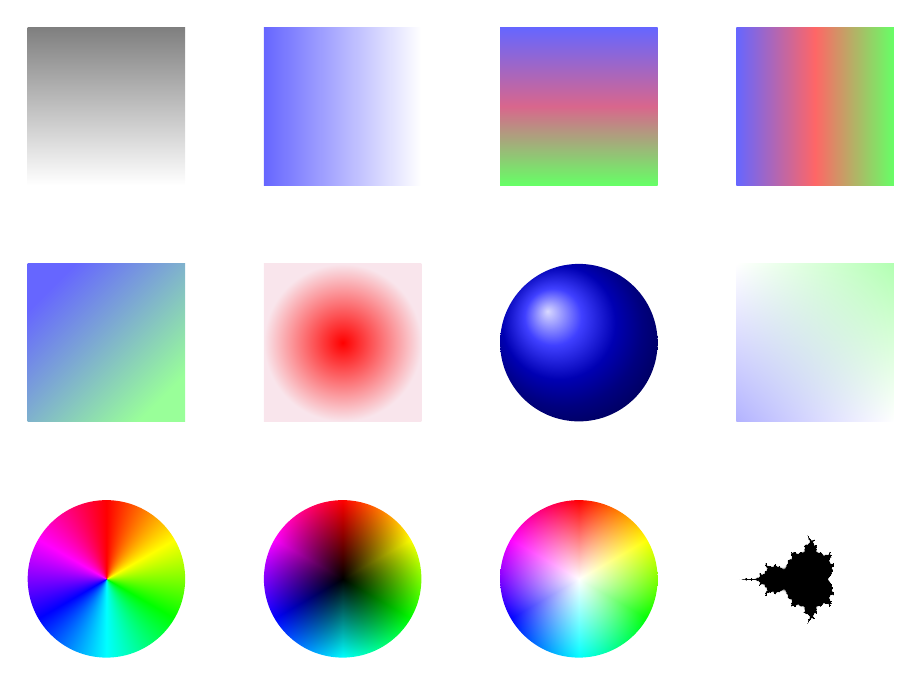
\begin{tikzpicture}
    %   \path[shade],可简写为\shade,需使用shadings库,可与draw参数一起使用. 参考15.7和 section 69
    %   1)axis模式, 左右或上下的线性颜色变化. 默认模式
    %     使用shading=axis指定模式,默认为从上到下,由灰色过渡到白色
    %     可使用如下参数: top color/bottom color/left color/right color/middle color
    %     middle color可结合top color/bottom color, 成为垂直中间颜色; middle color也可结合left color/right color, 成为水平中间颜色. middle color必须在top/bottom/left/right color之后使用
    %     shading angle可用于基于top/bottom旋转渐变方向,left/right默认为90
    \shade (0,0) rectangle (2,2);
    \shade[xshift=3cm,left color=blue!60] (0,0) rectangle (2,2);
    \shade[xshift=6cm,top color=blue!60,bottom color=green!60,middle color=purple!60] (0,0) rectangle (2,2);
    \shade[xshift=9cm,left color=blue!60,right color=green!60,middle color=red!60] (0,0) rectangle (2,2);
    \shade[yshift=-3cm,left color=blue!60,right color=green!40,shading angle=45] (0,0) rectangle (2,2);

    %   2)radial模式,由一点以半径向外扩散转化颜色
    %     使用shading=radial指定模式
    %     使用inner color指定中心颜色,outer color指定边缘颜色. 默认圆心为灰色,边缘颜色为白色
    \shade[shift={(3,-3)},shading=radial,inner color=red,outer color=purple!10] (0,0) rectangle (2,2);

    %   3)ball模式, 球体光影变化
    %     使用shading=ball指定模式,默认为蓝色
    %     可使用ball color指定颜色
    \shade[shift={(6,-3)},shading=ball] (1,1) circle [radius=1cm];

    %   4)bilinear interpolation模式,双线性
    %     使用shading=bilinear interpolation指定模式,需要导入shadings tikz库
    %     可使用以下关键字指定左上/右上/左下/右下颜色: upper left/upper right/lower left/lower right,默认都为白色
    \shade[shift={(9,-3)},shading=bilinear interpolation,upper right=green!30,lower left=blue!30] (0,0) rectangle (2,2);

    %   5)color wheel模式,车轮式颜色轮替
    %     使用shading=color wheel指定模式,需要导入shadings tikz库
    \shade[yshift=-6cm,shading=color wheel] (1,1) circle [radius=1cm];

    %   6)color wheel black center模式,车轮式颜色轮替,中心为黑色
    %     使用shading=color wheel black center指定模式,需要导入shadings tikz库
    \shade[shift={(3,-6)},shading=color wheel black center] (1,1) circle [radius=1cm];
    
    %   7)color wheel white center模式,车轮式颜色轮替,中心为白色
    %     使用shading=color wheel white center指定模式,需要导入shadings tikz库
    \shade[shift={(6,-6)},shading=color wheel white center] (1,1) circle [radius=1cm];

    %   8)Mandelbrot set模式,趣味性形状
    %     使用shading=Mandelbrot set指定模式,需要导入shadings tikz库
    \shade[shift={(9,-6)},shading=Mandelbrot set] (0,0) rectangle (2,2);
\end{tikzpicture}\newpage

%   9)结合透明模式. 需要导入fading tikz库
\begin{tikzfadingfrompicture}[name=fade rectangle]
    \shade[top color=transparent!100,bottom color=transparent!0] (0,0) rectangle (2,2);
\end{tikzfadingfrompicture}
\begin{tikzpicture}
    \fill [black!20] (-1.2,-1.2) rectangle (1.2,1.2);
    \pattern[pattern=checkerboard,pattern color=black!30] (-1.2,-1.2) rectangle (1.2,1.2);
    \fill[path fading=fade rectangle,red] (-1,-1) rectangle (1,1);
\end{tikzpicture}



% 4.使用预定义图形进行填充, 需要使用patterns库
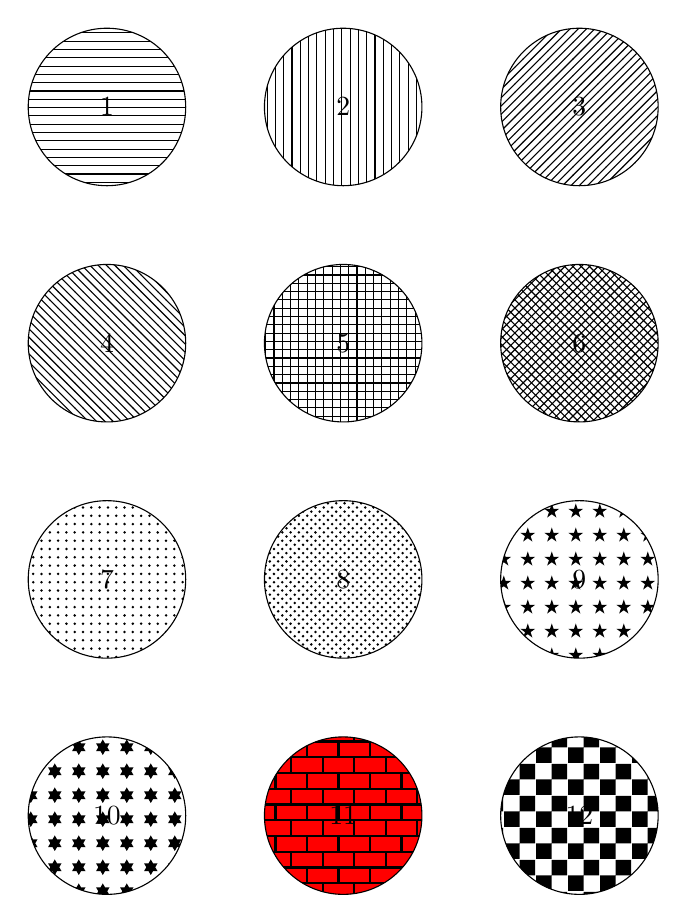
\begin{tikzpicture}
    %   \path[pattern]指定填充, 可简写为\pattern(section 62),可与draw参数一起使用
    %   如需填充空白区域,需要使用save path和use path,先对path fill,再pattern
    %   相关参数:
    %     pattern - 指定填充图形
    %     pattern color - 指定填充图形的颜色
    % 1) 水平线
    \path[draw,pattern=horizontal lines] (0,0) circle [radius=1cm];
    \node at (0,0){1};
    % 2)竖直线
    \draw[pattern=vertical lines,xshift=3cm] (0,0) circle [radius=1cm];
    \node[xshift=3cm] at (0,0){2};
    % 3)往东北的线
    \draw[pattern=north east lines,xshift=6cm] (0,0) circle [radius=1cm];
    \node[xshift=6cm] at (0,0){3};
    % 4)往东南的线
    \draw[pattern=north west lines,yshift=-3cm] (0,0) circle [radius=1cm];
    \node[yshift=-3cm] at (0,0){4};
    % 5)水平和竖直交叉线
    \draw[pattern=grid,shift={(3cm,-3cm)}] (0,0) circle [radius=1cm];
    \node[shift={(3cm,-3cm)}] at (0,0){5};
    % 6)东北和东南交叉线
    \draw[pattern=crosshatch,shift={(6cm,-3cm)}] (0,0) circle [radius=1cm];
    \node[shift={(6cm,-3cm)}] at (0,0){6};
    % 7)水平点阵
    \draw[pattern=dots,yshift=-6cm] (0,0) circle [radius=1cm];
    \node[yshift=-6cm] at (0,0){7};
    % 8)倾斜点阵
    \draw[pattern=crosshatch dots,shift={(3cm,-6cm)}] (0,0) circle [radius=1cm];
    \node[shift={(3cm,-6cm)}] at (0,0){8};
    % 9)五角星
    \draw[pattern=fivepointed stars,shift={(6cm,-6cm)}] (0,0) circle [radius=1cm];
    \node[shift={(6cm,-6cm)}] at (0,0){9};
    % 10)六角星
    \draw[pattern=sixpointed stars,yshift=-9cm] (0,0) circle [radius=1cm];
    \node[yshift=-9cm] at (0,0){10};
    % 11)砌砖块
    \path[save path=\pathA,shift={(3cm,-9cm)}] (0,0) circle [radius=1cm];
    \fill[red,use path=\pathA];
    \draw[pattern=bricks,use path=\pathA] ;
    \node[shift={(3cm,-9cm)}] at (0,0){11};
    % 12)黑白正方形间隔
    \draw[pattern=checkerboard,shift={(6cm,-9cm)}] (0,0) circle [radius=1cm];
    \node[shift={(6cm,-9cm)}] at (0,0){12};
\end{tikzpicture}\newpage


% 5.对之后的内容,作区域保留;之前的内容,不作区域限制
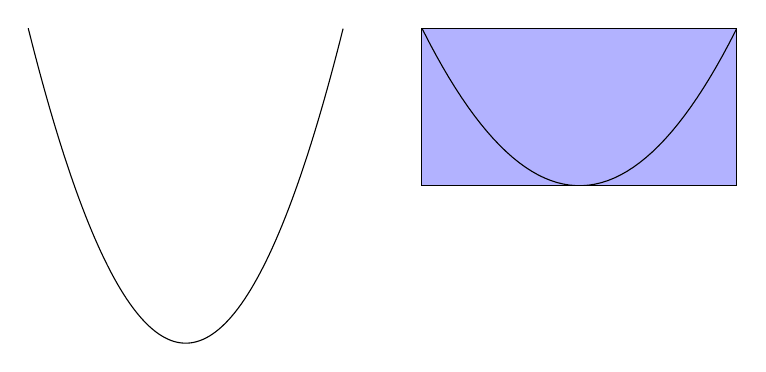
\begin{tikzpicture}
    %   \path[clip],可简写为\clip
    \begin{scope}[shift={(5cm,2cm)},scale=2,fill=blue!30]
        \path[fill,draw,clip] (-1,0) rectangle (1,1);
        \path[draw] plot[samples=100,domain=-2:2] (\x,\x*\x);
    \end{scope}
    \path[draw] plot[samples=100,domain=-2:2] (\x,\x*\x);
\end{tikzpicture}\newpage



% 连线类型-I
% 1.move to
%   (<coordinate_01>) (<coordinate_02>)
%   代表两点之间不连接,直接由上一个点,跳到下一个点
\begin{tikzpicture}
    \draw (0,0) -- (1,0) (2,0) -- (3,0);
\end{tikzpicture}


% 2.line to
%   (<coordinate>) -- (<coordinate>)
%   代表两点之间使用直线连接. 通常结尾使用cycle,使线条闭合
%   
% 3.(p) |- (q)
%   分别取坐标p的x值,坐标q的y值,组成(x,y),并依次连接(p) -- (x,y) -- (q)
%   (p) -| (q)
%   分别取坐标p的y值,坐标q的x值,组成(x,y),并依次连接(p) -- (x,y) -- (q)
\begin{tikzpicture}
    \begin{scope}[line width=2pt,yshift=-2cm]
        \draw (0,0) -- (1,0) -- (0,1) -- cycle;
        \draw[xshift=4cm] (0,0) -- (1,0) -- (0,1) -- (0,0);
    \end{scope}

    \begin{scope}[yshift=-4cm]
        \draw[->] (-1.5,0) -- (1.5,0) node[below]{$x$};
        \draw[->] (0,-1.5) -- (0,1.5) node[left]{$y$};
        \draw[red] (0,0) -| (1,1);
    \end{scope}
\end{tikzpicture}\vspace{1cm}


% 4.curve to
%   (<first_point>) .. controls (<first_control_point>) and (<second_control_point>) .. (<second_point>)
%   原理: 第一个点first_point的切线指向第一个控制点first_control_point,第二个点second_point的切线指向第二个控制点second_control_point
%   如果省略 and (<second_control_point>),则第二个点second_point的切线也指向第一个控制点first_control_point
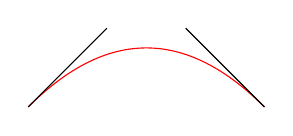
\begin{tikzpicture}
    \draw[red] (0,0) .. controls (1,1) and (2,1) .. (3,0);
    \draw (0,0) -- (1,1) (2,1) -- (3,0);
\end{tikzpicture}


% 连线类型-II
\begin{tikzpicture}
    % 5.抛物线(parabola)
    %   (<coordinate_01>) parabola (<coordinate_02>)
    %   从点coordinate_01到coordinate_02作抛物线,默认以coordinate_01作为抛物线顶点. 配合参数如下:
    %     bend - 指定弯曲坐标(即抛物线的顶点). 注意,线条必经过coordinate_01、bend点、coordinate_02,如果没有抛物线能满足该条件,则该线条不为抛物线
    %     bend pos - 弯曲点相对于coordinate_01到coordinate_02的相对分数点,需配合bend={+(<coordinate>)},相对于百分点位置移动的坐标
    %     parabola height - bend pos=0.5,bend={+{0,height}}的简便形式
    %     bend at start - 起始点坐标作为顶点
    %     bend at end - 结束点坐标作为顶点 
    \draw[->] (-3,0) -- (3,0) node[below]{$x$};
    \draw[->] (0,-3) -- (0,3) node[left]{$y$};
    \draw[red!50] (0,0) parabola[bend pos=0.5,bend={+(0,2)}] (2,0);
    \draw[blue!50] (0,0) parabola[bend={(-1,-2)}] (-2,0);
\end{tikzpicture}


\begin{tikzpicture}
    % <point1> to[out] <point2>
    %   在point1到point2的路径中,point1切线的倾斜角
    % <point1> to[in] <point2>
    %   在point1到point2的路径中,point2切线的倾斜角
    % <point1> to[out,relative] <point2>
    %   在point1到point2的路径中,point1切线的倾斜角相对于point1和point2连线的角度
    \draw (0,0) to[out=45,in=135] (1,0);
    \draw (2,0) to[out=45,in=135] (2,1);
    \draw (4,0) to[relative,out=45,in=135] (4,1);

    % <point1> to[bend left=<angle>] <point2>
    %    相当于out=<angle>,in=180-<angle>,relative
    % <point1> to[bend right=<angle>] <point2>
    %    相当于out=-<angle>,in=180+<angle>,relative
    \draw (6,0) to[bend left=30] (6,1);
    \draw (8,0) to[bend right=30] (8,1);
\end{tikzpicture}
    


% 图形形状
\begin{tikzpicture}
    % 1.圆(circle)
    %   (<central>) circle [radius=<radius>], 配合参数如下:
    %     x radius - x轴上的半径
    %     y radius - y轴上的半径
    %     radius - x/y轴上的半径
    %     at - 指定圆中心,不再将central作为圆中心
    \draw (2,0) circle [at={(0,0)},x radius=2,y radius=1];
    \draw (0,0) circle [radius=2pt];
    
    % 2.椭圆(ellipse)
    %   (<central>) circle [x radius=<x_radius>,y radius=<y_radius>], 配合参数如下:
    %     x radius - x轴上的半径
    %     y radius - y轴上的半径
    %     radius - x/y轴上的半径
    %     at - 指定椭圆中心,不再将central作为椭圆中心
    \draw (3,0) ellipse [x radius=1,y radius=0.5];

    % 3.长方形(rectangle)
    %   (<coordinate>) rectangle (<diagonal_coordinate>)
    \draw (5,-1) rectangle (7,1);

    % 4.(椭)圆弧(arc)
    %   (<start_point_coordinate>) arc [start angle=<start_angle>,end angle=<end_angle>,radius=<radius>], 配合参数如下:
    %     start_point_coordinate作为圆弧起点坐标,而非圆弧中心的坐标
    %     start angle - 起始角度
    %     end angle - 结束角度
    %     delta angle - 起始角度与结束角度的差值
    %     ** 如果start angle和delta angle被指定,则end = start + delta
    %     ** 如果end angle和delta angle被指定,则start = end - delta
    %     ** 如果start angle/end angle/delta angle被同时指定,delta angle被忽略
    %     x radius - x轴上的半径
    %     y radius - y轴上的半径
    %     radius - x/y轴上的半径
    \draw (1,-3) arc [start angle=0,end angle=180,radius=1];
    
    % 5.辅助网格(grid)
    %   (<coordinate>) grid (<diagonal_coordinate>), 配合参数如下:
    %     xstep - 指定x轴上的步进. 如果xstep单位为纯数字,则使用x轴默认长度,factor(xstep) * default_length; 如果为dimension,则使用指定长度作为步进. 默认为1cm
    %     ystep - 指定y轴上的步进. 参考xtep
    %     step - 指定x/y轴上的步进. 参考xstep
    %     ** grid是基于原点(0,0)向外拓展的
    \begin{scope}[shift={(4,-4)}]
        \draw[->] (-2cm,0) -- (2cm,0) node[below]{$x$};
        \draw[->] (0,-2cm) -- (0,2cm) node[left]{$y$};
        \draw (-1,-1) grid[step=0.5] (0,0);
        \draw (0,0) grid[step=5mm] (1,1);
    \end{scope}
\end{tikzpicture}



% 图形属性
% 1.填充颜色: 已定义颜色和颜色表达式,可使用latex的xcolor宏包(只支持gray/rgb/RGB颜色模型)
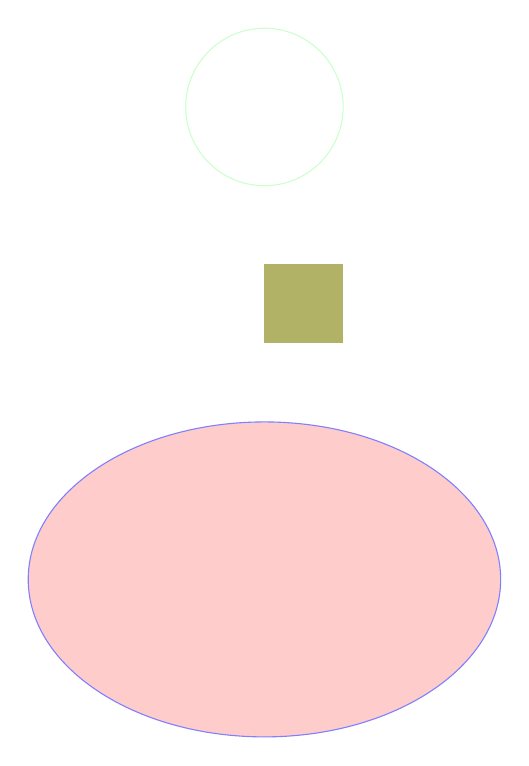
\begin{tikzpicture}
    % draw中, color指定边框颜色
    \draw[color=green!20] (0,3) circle [radius=1cm];
    % fill中, color指定填充颜色
    \fill[color=red!50!green!60] (0,0) rectangle (1,1);
    % filldraw中,color指定填充和边框颜色,fill指定填充颜色,draw指定边框颜色
    \filldraw[color=blue!50,fill=red!20] (0,-3) ellipse [x radius=3cm,y radius=2cm];
\end{tikzpicture}\vspace{1cm}


% 2.坐标顶点是圆角/尖角
\begin{tikzpicture}
    % rounded corners=<dimension>
    %   圆滑的边角弧度,dimension值不被scale影响
    % sharp corners
    %   尖锐的边角弧度
    % 可以在路径中使用,影响后续顶点弧度
    \draw (0,0) -- (2,0) -- (2,1) -- (0,1) -- cycle;
    \draw[xshift=4cm,rounded corners=5pt] (0,0) -- (2,0) -- (2,1) -- (0,1) -- cycle;
    \draw[yshift=-2cm] (0,0) -- (2,0) -- (2,1) [rounded corners=5pt] -- (0,1) -- cycle;
\end{tikzpicture}


% 3.保存/取用路径
%   save path - 保存路径到宏(类似于命令格式,需要反斜杠开头)
%   use path - 取用路径
\begin{tikzpicture}[>=stealth]
    \path[save path=\pathA] (0,0) -- (1,0);
    \draw[red,use path=\pathA];
\end{tikzpicture}


% 4.线条粗细 

\begin{tikzpicture}
    % 1)line width=<dimension>
    %   指定线条宽度尺寸
    % 2)使用预定义宽度: 
    %   [1]ultra thin(0.1pt)
    \draw[ultra thin] (-2,1) -- (2,1);
    %   [2]very thin(0.2pt)
    \draw[very thin] (-2,0.5) -- (2,0.5);
    %   [3]thin(默认,即0.4pt)
    \draw[thin] (-2,0) -- (2,0);
    \draw (-2,-0.5) -- (2,-0.5);
    %   [4]semithick(0.6pt)
    \draw[semithick] (-2,-1) -- (2,-1);
    %   [5]thick(0.8pt)
    \draw[thick] (-2,-1.5) -- (2,-1.5);
    %   [6]very thick(1.2pt)
    \draw[very thick] (-2,-2) -- (2,-2);
    %   [7]ultra thick(1.6pt)
    \draw[ultra thick] (-2,-2.5) -- (2,-2.5);
\end{tikzpicture}\newpage


% 5.线条端点风格

\begin{tikzpicture}
    \begin{scope}[line width=10pt]
        % 1)round - 圆润端点
        \draw[line cap=round] (0,1 ) -- +(1,0);
        % 2)butt - 尖锐端点(无延长)
        \draw[line cap=butt] (0,.5) -- +(1,0);
        % 3)rect - 尖锐端点(延长)
        \draw[line cap=rect] (0,0 ) -- +(1,0);
    \end{scope}
    \draw[white,line width=1pt] (0,0 ) -- +(1,0) (0,.5) -- +(1,0) (0,1 ) -- +(1,0);
\end{tikzpicture}


% 6.线条相交风格
\begin{tikzpicture}[line width=10pt]
    1)round - 圆润
    \draw[line join=round] (0,0) -- ++(.5,1) -- ++(.5,-1);
    2)bevel - 平折型
    \draw[line join=bevel] (1.25,0) -- ++(.5,1) -- ++(.5,-1);
    3)miter - 尖锐型
    \draw[line join=miter] (2.5,0) -- ++(.5,1) -- ++(.5,-1);
\end{tikzpicture}

% 7.线条类型: tikz的线条主要由虚线来实现
\begin{tikzpicture}[|-|]
    % 1)dash pattern=on 2pt off 3pt on 4pt off 4pt
    %   代表画2pt线条,间隔3pt,再画4pt线条,再间隔4pt
    % 2)dash phase=3pt
    %   将通过dash pattern配置的虚线,左移3pt
    % 3)dash=<pattern> phase <phase>
    %   合并1/2步
    % 4)dash expand off
    %   在只有一个on和一个off的dash pattern中,off部分可适应性延伸. 需要decorations tikz库
    % 5)其他预定义线条
    %   [1]solid - 实线. 默认类型
    %   [2]dotted/densely dotted/loosely dotted - 点线/密集点线/稀疏点线
    %   [3]dashed/densely dashed/loosely dashed - 虚线/密集虚线/稀疏虚线
    %   [4]dash dot/densely dash dot/loosely dash dot - 虚点线/密集虚点线/稀疏虚点线
    %   [5]dash dot dot/densely dash dot dot/loosely dash dot dot - 虚点点线/密集虚点点线/稀疏虚点点线
    \draw[dash pattern=on 2pt off 2pt] (-2,0) -- ++(4,0);
    \draw[dash pattern=on 2pt off 2pt,dash phase=3pt] (-2,-1) -- ++(4,0);
    \draw[dash pattern=on 2pt off 2pt,dash expand off] (-2,-2) -- ++(4,0);
    \draw[dash pattern=on 2pt off 2pt,dash expand off] (-2,-3) -- ++(3.9,0);
    \draw[dash pattern=on 2pt off 2pt,dash expand off] (-2,-4) -- ++(3.8,0);
    \draw[dash pattern=on 2pt off 2pt,dash expand off] (-2,-5) -- ++(3.7,0);
\end{tikzpicture}


% 8.双边框线

\begin{tikzpicture}
    % 实现原理: 使边框线条加粗,然后再次画一条相交于边框线更细的线. 此时line width为单一分部的宽度
    % 1)double - 画细线,可指定细线的颜色. 默认细线颜色为白色
    % 2)double distance - 指定细线的宽度(粗线两分部的内部距). 默认0.6pt
    % 3)double distance between line centers - 指定细线的宽度(粗线两分部的中心距)
    \draw[line width=10pt,double distance between line centers=10pt] (-2,0) -- ++(4,0);
    \draw[red,line width=10pt,double distance=10pt] (-2,-2) -- ++(4,0);
\end{tikzpicture}


% 9.在当前路径闭合区域填充自定义内容
\begin{tikzpicture}
    % path picture - 指定填充的自定义内容. 使用预定义参数path picture bounding box引用闭合路径
    \draw[path picture={
        \node at (path picture bounding box.center){
\includegraphics[scale=0.6]{pic/dog_01.png}};
    }] (0,0) circle [radius=2];
\end{tikzpicture}


% 10.边界盒子
%   1)默认边界盒子随着作图过程,取所有路径中最外部的x/y的上下限值,作为边界盒子的边界
%     使用预定义变量current bounding box获得当前边界盒子
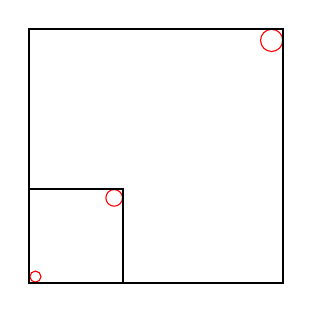
\begin{tikzpicture}
    \draw[red] (0,0) circle (2pt);
    \draw[red] (1,1) circle (3pt);
    \draw (current bounding box.south west) rectangle (current bounding box.north east);
    \draw[red] (3,3) circle (4pt);
    \draw[thick] (current bounding box.south west) rectangle (current bounding box.north east);
\end{tikzpicture}\vspace{1cm}

%   2)use as bounding box - 只参考指定路径作为边界盒子参考值
Left of picture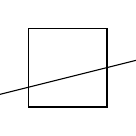
\begin{tikzpicture}
    \draw[use as bounding box] (2,0) rectangle (3,1);
    \draw (1,0) -- (4,.75);
\end{tikzpicture}right of picture.\\

Left of picture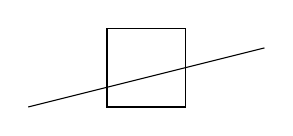
\begin{tikzpicture}
    \draw (2,0) rectangle (3,1);
    \draw (1,0) -- (4,.75);
\end{tikzpicture}right of picture.\\[1cm]

%   3)如果前面已有路径,边界比当前使用use as bounding box的路径更偏向外部,则无法生效. 使用\pgfresetboundingbox
Left of picture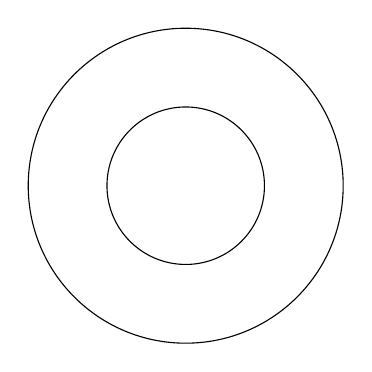
\begin{tikzpicture}
    \draw (0,0) circle [radius=2];
    \draw[use as bounding box] (0,0) circle [radius=1];
\end{tikzpicture}right of picture.\\[3cm]

Left of picture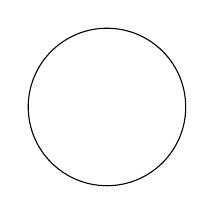
\begin{tikzpicture}
    \draw (0,0) circle [radius=2];
    \pgfresetboundingbox
    \draw[use as bounding box] (0,0) circle [radius=1];
\end{tikzpicture}right of picture.\\

%   4)trim left - 将指定x值的左侧视为bounding box外部内容. 参数可以为dimension或point,point取x值
%   5)trim right - 将指定x值的右侧视为bounding box外部内容. 参数可以为dimension或point,point取x值
Left of picture\begin{tikzpicture}[trim left=0]
    \draw (0,0) circle [radius=2];
\end{tikzpicture}right of picture.\\[3cm]

Left of picture\begin{tikzpicture}[trim right=0]
    \draw (0,0) circle [radius=2];
\end{tikzpicture}right of picture.\\


% 11.参数的执行顺序
%   preaction -- normal -- postaction
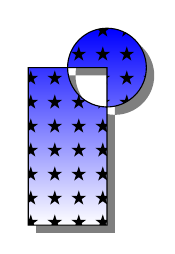
\begin{tikzpicture}
    \draw[preaction={fill=black,opacity=0.5,transform canvas={xshift=1mm,yshift=-1mm}}]
    [preaction={top color=blue,bottom color=white}]
    [pattern=fivepointed stars]
    (0,0) rectangle (1,2)
    (1,2) circle [radius=5mm];
\end{tikzpicture}


% 12.路径装饰,参考section 24和section 50
% decoration类型:
%   1)path morphing
%     将原来的一条path,转化为一条path. 需要调用decorations.pathmorphing库
%     path morphing列表:
%     [1]lineto - 直线
%     [2]curveto - 曲线
%     [3]random steps - 随机步. 可使用参数:
%       segment length - 周期长度
%       amplitude - 振幅 
%     [4]saw - 锯齿. 可使用参数:
%       segment length - 周期长度
%       amplitude - 振幅        
%     [5]zigzag - Z字形. 可使用参数:
%       segment length - 周期长度
%       amplitude - 振幅   
%     [6]bent - 弯曲形. 可使用参数:
%       aspect - 线条紧绷度. 0.3左右最合适
%       amplitude - 振幅   
%     [7]bumps - 半椭圆. 可使用参数:
%       segment length - 椭圆宽度半径
%       amplitude - 椭圆高度半径 
%     [8]coil - 线圈. 可使用参数:
%       segment length - 线圈周期半径
%       amplitude - 线圈半径
%       aspect - 观测角度. 0代表从侧面看,1代表从正面看
%     [9]snake - 蛇形曲线. 可使用参数:
%       segment length - 周期长度
%       amplitude - 振幅
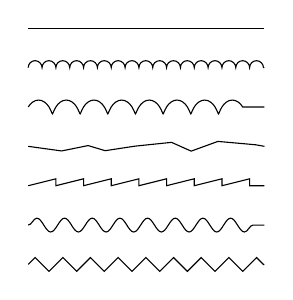
\begin{tikzpicture}
    \draw (0,0) -- ++(3,0);
    \draw[decorate,decoration=bumps] (0,-0.5) -- ++(3,0);
    \draw[decorate,decoration=coil] (0,-1) -- ++(3,0);
    \draw[decorate,decoration=random steps] (0,-1.5) -- ++(3,0);
    \draw[decorate,decoration=saw] (0,-2) -- ++(3,0);
    \draw[decorate,decoration=snake] (0,-2.5) -- ++(3,0);
    \draw[decorate,decoration=zigzag] (0,-3) -- ++(3,0);
\end{tikzpicture}

%   2)path replacing
%     将原来的一条path,转化为一系列不相连的短path. 需调用decorations.pathreplacing和decorations.shapes库
%     decorations.pathreplacing列表:
%     [1]moveto - 跳转线
%     [2]border - 边界标记线. 可使用参数:
%       segment length - 两个标记线之间的距离
%       amplitude - 标记线长度
%       angle - 标记线与路径的夹角
%     [3]brace - 大括号. 可使用参数:
%       amplitude - 大括号的高度
%       aspect - 大括号中点的位置. 0位于起始点,1位于结束点
%     [4]expanding waves - 逐渐增大的波纹. 可使用参数:
%       segment length - 波纹之间的距离
%       angle - 波纹的圆心角的一半
%     [5]ticks - 垂直于路径切线的直线. 可使用参数:
%       segment length - 直线之间的距离
%       amplitude - 直线长度的一半
%     [6]waves - 固定大小的圆弧. 可使用参数:
%       segment length - 圆弧之间的距离
%       angle - 圆弧圆心角的一半
%       radius - 圆弧的半径
%     decorations.footprints列表:
%       footprints
%         脚印. 相关参数:
%           [1]foot length - 脚印长度. 默认10pt
%           [2]stride length - 左脚脚后跟到下一个左脚脚后跟的距离. 默认30pt
%           [3]foot sep - 左脚与右脚之间的间隔. 默认4pt
%           [4]foot angle - 脚印偏离path的角度. 默认10
%           [5]foot of - 指定脚印类别. 列表:gnome/human(默认)/bird/felis silvestris
%     decorations.shapes列表:
%       [1]crosses - 交叉线. 可使用参数:
%         segment length - 交叉线中心的间隔
%         shape width - 交叉线的宽度
%         shape height - 交叉线的高度
%       [2]triangles - 三角形. 可使用参数:
%         segment length - 三角形的间隔
%         shape width - 三角形的宽度
%         shape height - 三角形的高度
\begin{tikzpicture}
    \draw[decorate,decoration=brace] (0,-0.5) -- ++(3,0);
    \draw[decorate,decoration=crosses] (0,-1) -- ++(3,0);
    \draw[decorate,decoration=ticks] (0,-1.5) -- ++(3,0);
    \draw[decorate,decoration=expanding waves] (0,-4) -- ++(3,0);
    \draw[decorate,decoration=triangles] (0,-6.5) -- ++(3,0);
    \draw[decorate,decoration=shape backgrounds] (0,-7) -- ++(3,0);
\end{tikzpicture}

%   3)path removing
%     将原来的一条path,进行移除,添加文字. 需调用decorations.text库
%     decorations.text列表:
%     [1]text along path - 沿path的文本. 相关参数:
%       text=<text>
%         顺着path的文本内容. text相关:
%           i.使用\<space>添加额外空格
%           ii.指定text的格式,需要用分隔符来区分. 如: 当text format delimiters={[}{]},[\color{red}]see you again[]用于指定部分字体颜色为红色
%       text format delimiters={<start>}{<end>}
%         指定text部分格式的分隔符
%       text color=<color>
%         指定text字体颜色
%       reverse path=<boolean>
%         在排列text时,将path视为反方向
%       text align={<options>}
%         将text沿指定位置对齐. 参数列表如下:
%           align=<direction>
%           对齐位置. 列表如下:
%             left - 沿path起始位置
%             right - 沿path结束位置
%             center - 沿path中间位置居中对齐
%           left indent=<length>
%           当align=left,沿path起始位置的缩进
%           right indent=<length>
%           当align=right,沿path结束位置的缩进
%           fit to path=<boolean>
%           将text伸缩以适配path长度. 伸缩字符之间的间隙
%           fit to path stretching spaces=<boolean>
%           将text伸缩以适配path长度. 只伸缩单词之间的空格
\begin{tikzpicture}
    \draw[postaction={decorate,decoration={text along path,raise=-8pt,text={try your best,enjoy your lift,love your parents}}}] (0,0) circle [radius=2];
\end{tikzpicture}

%     [2]text effects along path
%       类似于text along path,但当前类型的每一个字符都是node,可以使用node的参数

% decoration语法
%   1)\path[decorate,decoration] <path>
%     对整段path进行decorate
%   2)\path decorate[decoration] {<path>}
%     对subpath进行decorate,并且可嵌套(嵌套需要内层为path morphing,外层为path replacing)

% 参数
%   1)decorate - 路径为装饰符格式
%   2)decoration=<options>
%     指定装饰符. 相关参数如下
%     [1]name - 引用的装饰符名称. 如: name=brace
%     [2]mirror - 关于原path的镜像
%     [3]raise - 往原path路径方向的左侧偏移
%     [4]transform - 对decoration进行shift或rotate操作
%     [5]pre - 在起始的地方使用指定线条或decorate. 可使用lineto/moveto/curveto或decoration
%     [6]pre length - 在起始指定长度使用指定线条
%     [7]post - 在结束的地方使用指定线条或decorate. 可使用lineto/moveto/curveto或decoration
%     [8]post length - 在结束指定长度使用指定线条
%     [9]segment length - 一个周期的长度
%     [10]amplitude - 振幅(波峰到平衡位置的距离)
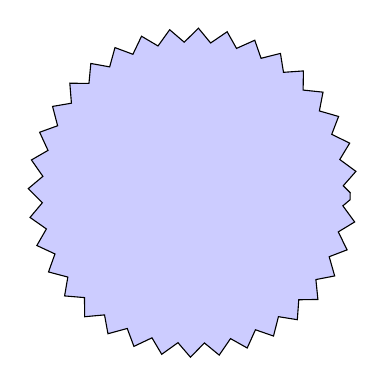
\begin{tikzpicture}
    \draw[fill=blue!20,decorate,decoration=zigzag] (0,0) circle [radius=2];
\end{tikzpicture}


% 13.透明度,范围[0,1],0代表完全透明,1代表完全不透明

\begin{tikzpicture}
    % draw中,opacity指定边框透明度
    % fill中,opacity指定填充透明度
    % filldraw中,fill opacity指定填充透明度,draw opacity指定边框透明度,opacity指定填充和边框透明度
    \draw[line width=6pt,green!50,opacity=0.6] (1,0) circle [radius=1];
    \fill[opacity=0.6,blue!50] (1,-3) circle [radius=1];
    \filldraw[fill opacity=0.2,fill=blue!50,draw opacity=0.4,draw=green,line width=20pt] (1,-6) circle [radius=1];
    \filldraw[opacity=0.2,line width=20pt] (1,-9) circle [radius=0.5];
\end{tikzpicture}

% update 2025-04-19
\end{document}
